\documentclass[12pt,a4paper]{report}

\renewcommand{\familydefault}{\sfdefault}

\usepackage[pdftex]{graphicx}
\usepackage{float}
\usepackage{fancyvrb}
\usepackage{minted}
\usepackage[utf8]{inputenc}
\usepackage[portuges]{babel}
\usepackage[T1]{fontenc}
\usepackage{times}
\usepackage[left=30mm,right=25mm,top=30mm,bottom=25mm,headsep=1.3cm]{geometry}
\usepackage{titlesec}
\usepackage{mathtools}
\usepackage{indentfirst}
\usepackage{enumerate}
\usepackage{amsfonts}
\usepackage{fancyhdr}
\usepackage{amsfonts}
\usepackage{tabu}
\usepackage{multicol}
\usepackage[table,xcdraw]{xcolor}
\usepackage{subfigure}
\usepackage{url}
\usepackage{hyperref}
\usepackage{enumitem}
\titlespacing*{\chapter}{0pt}{-0pt}{30pt}

\fancypagestyle{plain}{}
\pagestyle{fancy}
\fancyhead[L]{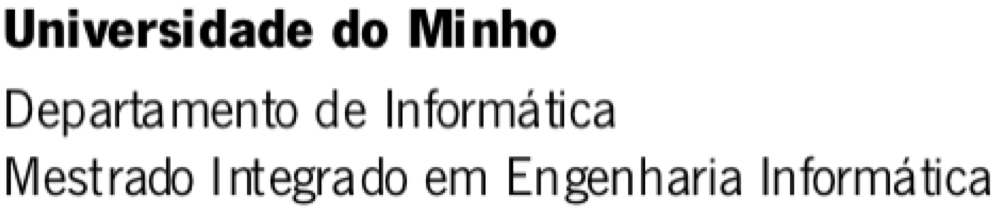
\includegraphics[scale=0.3]{Imagens/logoPB.png}}
\fancyhead[R]{Classificação Emotiva de Texto - CN}

\AtBeginEnvironment{minted}{\fontsize{11}{11}\selectfont}

\newcommand{\HRule}{\rule{\linewidth}{0.5mm}}
\titleformat{\chapter}{\bfseries\huge}{\thechapter.}{20pt}{\huge}


\begin{document}

\begin{titlepage}

\newgeometry{left=5cm,top=0cm}

\begin{minipage}{0.6\textwidth}
\begin{flushleft} 

\includegraphics[width=\textwidth]{./Imagens/logo.png}
\end{flushleft}
\end{minipage}

\vspace{3cm}

\Huge

\textbf{Diagnóstico de um Projeto Ágil}

\LARGE

Gestão de Processo de Software 

\vfill

\normalsize

\textbf{Grupo de trabalho:}

Rogério Gomes Lopes Moreira, A74634

Samuel Gonçalves Ferreira, A76507

\vspace{5mm}

\textbf{Docente:}

Pedro Miguel Gonzalez Abreu Ribeiro


\vfill

Braga, {\today}

\end{titlepage}

\restoregeometry

\tableofcontents

\begin{abstract}

Com o massivo volume de publicações que diariamente se realizam nas diversas redes sociais, torna-se relevante realizar uma análise de alto nível do seu conteúdo.
Aliando esta fonte de dados à atual capacidade de processamento que se consegue obter em métodos de \textit{Machine Learning} é assim viável a exploração destes dados com base nestas técnicas, como forma de análise dos mesmos. 

Neste sentido, o presente projeto prático pretende explorar a utilização de \textit{Redes Neuronais Artificiais} (\textit{RNAs}) num problema de classificação emocional de texto, através de publicações na rede social \textit{Twitter}. 

Ao longo deste relatório é apresentado todo o processo desenvolvido como forma de analisar o conjunto de dados em bruto, o pré processamento do mesmo, o desenvolvimento da arquitetura da RNA e o processo de treino e teste da mesma. 

Por fim, são apresentados os resultados obtidos, focando os padrões de treino que obtêm melhores resultados de classificação. 

\end{abstract}
\chapter{Introdução}

Redes neuronais artificias apresentam-se como um sistema conexionista, fortemente inspirado nas características do sistema nervoso central do ser humano. 
Apesar das RNAs serem um modelo simplificado, a sua arquitetura extremamente interligada de unidades de processamento permite que estas sejam capazes de generalizar e adquirir conhecimento, através de um processo de aprendizagem. 

Tirando partidos das suas características, vários algoritmos de \textit{Machine Learning} recaem sobre estas estruturas de aprendizagem, devido às suas capacidades de classificação e previsão em qualquer um dos paradigmas de aprendizagem. 

Neste projeto procura-se assim recorrer às capacidades de uma RNA, criada e modelada ao contexto do problema, para realizar a classificação do nível emocional de publicações da rede social \textit{Twitter}. 

No sentido de introduzir e uniformizar os conceitos em torno das RNAs, o presente relatório fornece inicialmente um descrição teórica dos principais temas associados com a modelação de uma rede neuronal artificial. 
Posteriormente, são descritas todas as etapas desenvolvidas ao longo do projeto e as decisões tomadas no decorrer deste.

Como estrutura do presente documento: o capítulo \ref{chp:rna} apresenta uma descrição breve daquilo que atualmente se entende por uma rede neuronal artificial, focando com relevo as características das suas unidades de processamento (neurónios), as arquiteturas existentes e o algoritmo de aprendizagem de \textit{Back-Propagation}; o capítulo \ref{chp:AnaliseDados} apresenta uma descrição da fase de pré processamento dos dados, focando a eliminação de ruído, seleção da informação útil e criação de novos atributos.

De seguida, numa vertente mais prática, os capítulos \ref{chp:criacaoRNAs} e \ref{cht:analiseresultados} apresentam, respetivamente, todas as considerações no processo de desenvolvimento e análise de resultados, ao longo dos diferentes cenários de teste realizados. 

Por fim, o capítulo \ref{chp:conclusao} apresenta as conclusões relativamente ao projeto e o trabalho futuro. 

\vspace{5cm}




\chapter{Redes Neuronais Artificiais}
\label{chp:rna}

\section{Descrição geral}
\label{sec:RNA-Descricao}

Apresentando-se como uma abordagem de \textit{machine learning}, os algoritmos de redes neuronais artificias (RNAs) baseiam-se num sistema conexionista, inspirado no funcionamento da estrutura cerebral humana.

Estas técnicas recorrem a uma topologia em rede para receber informações que, após processadas, influenciam o estado interno de cada neurónio da rede.
O conhecimento é assim adquirido através do ambiente por um processo iterativo de aprendizagem. 
Este conhecimento é armazenado nas conexões da rede, através de uma adaptação dos pesos dos neurónios -ou nodos- ao longo de um processo de aprendizagem. 

Independente do contexto, uma rede neuronal apresenta uma arquitetura genérica (Figura \ref{fig:arquiteturas}), normalmente composta pelas seguintes camadas \cite{CortezNevesANN, ann-agility}: 
\begin{itemize}
    \item \textbf{Camada de entrada}, na qual é recebida a informação a analisar. 
    Apesar dos dados serem normalmente obtidos através de um dataset pré preparado, esta camada pode ser vista como a comunicação da rede com o ambiente, como forma de percecionar e obter dados. 
    
    É assim uma camada sem antecessor, servindo como uma interface para alimenta a rede com nova informação. 
    
    \item \textbf{Camadas intermédias}, que desempenham a tarefa de processamento dos dados de entrada, com base num determinado paradigma de aprendizagem. 
    
    \item \textbf{Camada de saída}, onde se devolvem os resultados do processo de aprendizagem da rede. 
    
    O número de nodos de saída está diretamente relacionado com o número de parâmetros que são previsto pela rede num determinado contexto. 
\end{itemize}

Alguns dos benefícios das redes neuronais, comparativamente a outros processos de \textit{Machine Learning}, estão associados ao seu puder de processamento. Esta capacidade deve-se essencialmente à sua estrutura, que permite executar um ambiente extremamente paralelo.
Além deste fator, apresentam ainda outras características de relevo, nomeadamente \cite{ann-agility}  \cite{CortezNevesANN} \cite{Haykin-ANN}:
\begin{itemize} 
    \item \textbf{Generalização}: No final do processo de aprendizagem, a rede é capaz de descrever um universo completo, através de uma aprendizagem prévia com algumas das suas partes. 
    Além disto, devido à sua robustez, as RNAs são ainda capazes de processar ruído ou informação incompleta, conseguindo generalizar a informação que analisam na fase de treino para novos casos futuros. 
    
    \item \textbf{Não linearidade}: Além de problemas simples, estes algoritmos apresentam-se capazes de analisar características não lineares, através da interconexão de diferentes neurónios e uso de diferentes funções de ativação; 
    
    \item \textbf{Relação entre input-output}: Quando aplicadas num contexto de aprendizagem supervisionada, com um conjunto de input de treino e um dataset de output esperado, as redes neuronais são capazes de gerar resultados satisfatórios de classificação;
    
    \item \textbf{Adaptação}: Uma das principais características das RNAs reside na sua capacidade de adaptação, útil em ambientes com dados desconhecidos ou em falta. 
    
    Os pesos atribuídos a cada neurónio são capazes de ser adaptar, conforme o domínio sobre a qual a rede se encontra a ser treinada. Alem disto, a sua topologia pode também alterar-se de acordo com as mudanças do ambiente, criando ou reduzindo o número de ligações entre nodos. 

    Desta forma, no final do processo de aprendizagem, uma RNA é capaz de generalizar novos casos à sua capacidade de raciocínio. 
    
    \item \textbf{Tolerância a falhas}: Devido à sua topologia, as RNAs permitem um elevada tolerância a falhas. 
    A falha de um neurónio pode ser atenuada pela marcação do peso dos seus axónios como zero, simulando assim o desaparecimento das ligações para aquele neurónio. 
    
    A falha de um neurónio leva ao reajustamento dos restantes, levando a uma degradação gradual e suave da rede, em caso de desativação de algumas conexões entre neurónios. 
\end{itemize}


\section{Neurónio Artificial}
\label{sec:Neuronio}

Cada camada de uma RNA é composta por um conjunto de neurónios, identificados pelos nodos da topologia da rede. 
Um neurónio pode ser visto como uma unidade de processamento da rede, recebendo ligações de outro neurónios e unindo-se a outros nodos da rede semelhantes a si. 

As ligações entre neurónios são designadas por axónios, tal como na estrutura biológica do cérebro e, têm a si associadas um peso. Este peso pode, numa interpretação simples, ser visto como a importância da informação que aquele axónio envia a um neurónio.
O peso de cada axónio é regulado ao longo do processo de aprendizagem, levando a uma generalização da topologia da rede aos dados, até se obter um resultado coerente com os esperados no contexto. 
A transmissão de informação entre os nodos é conseguida através de sinapses, novamente seguindo a nomenclatura biológica. 

Ao longo do processo de evolução da rede, os neurónios vão atualizando o seu estado, sendo este normalmente representado por um valor numérico entre \textit{[0, 1]}.
De uma forma geral, o estado interno de um neurónio é caracterizado por:
\begin{itemize} 
    \item Um \textbf{conjunto de ligações}, cada uma com o seu próprio peso. 
    Ao longo da evolução da rede, o sinal propagado por um determinado axónio é multiplicado pelo peso do mesmo, resultando assim na excitação -ou inibição- do nodo;

    \item Um \textbf{Integrador}: Apresenta-se como uma função de redução, que simplifica a influencia das N conexões de entrada de um neurónio para um único valor. 
    
    Geralmente, o integrador realiza apenas o somatório $(\sum)$ dos valores recebidos pelas N ligações de entrada, multiplicados pelo peso da respetiva ligação;
    
    \item A \textbf{Função de Ativação}: Determina o valor de saída do neurónio, de forma a restringir o valor de saída do neurónio para um determinado valor finito. 
    Este valor é normalmente calculado através do mapeamento do valor do integrador para uma determinada função não linear. De referir que a escolha da função de ativação tem uma influência direta e bastante significativa na capacidade de aprendizagem da rede.  
    
    Algumas das principais funções são a função binária (degrau), linear ou funções do tipo \textit{sigmoide}. \cite{ANN-chemiProb}
    Em pesquisas recentes, foi ainda apresentada a função designada por \textit{ReLU}. (Figura \ref{fig:act-func}) Esta função, explorada pelos investigadores da \textit{Google Brain Team}, apresenta algumas vantagens face a implementações com a função \textit{sigmoide}.

\end{itemize}

\begin{figure}
    \hspace{-0.2in}
    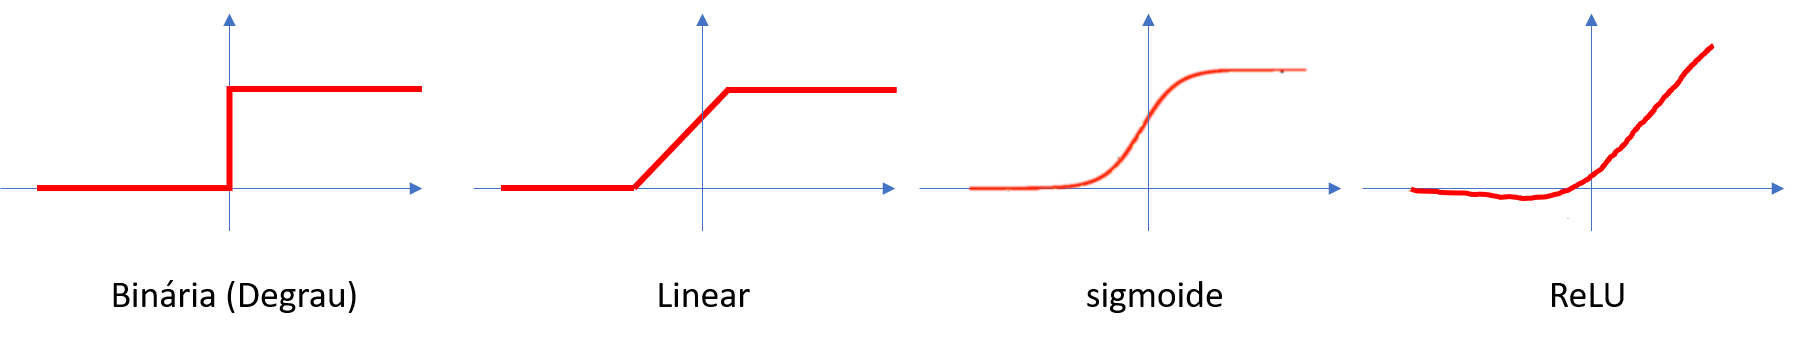
\includegraphics[scale=0.53]{Imagens/actfun.png}
    \caption{Exemplos de diferentes tipos de funções utilizadas como função de ativação dos neurónios.}
    \label{fig:act-func}
\end{figure}

\section{Arquiteturas da Rede }
\label{sec:Arquiteturas}

A arquitetura de uma rede neuronal artificial especifica a quantidade de neurónios (nodos) que a mesma possui e, de que formas estes se relacionam e interligam entre si.
A arquitetura pode ser visualizada na forma de grafos, no qual as ligações entre os nodos são orientadas. 

De uma forma geral existem três tipos distintos de topologia, sendo que quanto mais complexa a arquitetura de uma RNA, maior a sua capacidade para lidar com problemas mais complexos. 

\begin{itemize}
    \item \textbf{\textit{Single Layer Feedforward}}: As ligações da rede seguem apenas uma direção. Nesta arquitetura não existem camadas intermédias, existindo apenas as camadas de \textit{input} e \textit{output}. 
    
    A partir de um nodo de entrada existem apenas ligações divergentes (1 para N)  e os nodos de saída apresentam ligações convergentes (N para 1). Esta topologia representa as arquiteturas inicias das RNAs. (Figura \ref{fig:arquiteturas}-a)
    
    \item \textbf{\textit{Multi-Layer Feedforward}}: Seguindo os mesmos conceitos da arquitetura anterior, as RNAs \textit{multi-layer} permitem a definição de uma ou mais camadas intermédias. 
    Embora esta relação não seja linear, a adição de camadas intermédias a uma rede permite aumentar a sua capacidade de aprendizagem, podendo assim lidar com funções e relações entre os dados mais complexas. 
    
    Estas redes são assim úteis em contextos onde existe um grande número de dados de input, sobre os quais se espera observar alguma relação ou padrões gerais. Contudo, o aumento do número de camadas de uma rede neuronal, leva a um aumento exponencial do seu tempo de aprendizagem. (Figura \ref{fig:arquiteturas}-b)
    
    Neste tipo de arquiteturas, o algoritmo de \textit{Back-Propagation} é um dos principais métodos de aprendizagem. Este método calcula a contribuição do erro para cada um dos nodos da rede, ajustando o peso de cada nodo com base no erro calculado (Secção \ref{sec:backProp}). 

    \item \textbf{Redes recorrentes}: Numa sucessão à arquitetura anterior, as RNAs baseadas em  redes recorrentes permitam a existência de conexões de um nodo para si próprio. A ligação de um neurónio para si próprio permite a introdução de conceitos de “memória” no próprio nodo. 
    
    Além deste fator, um neurónio pode ainda ligar-se a outros nodos de camadas anteriores ou da própria camada, permitindo assim a existência de ciclos na estrutura. (Figura \ref{fig:arquiteturas}-c)
\end{itemize}

\begin{figure}
    \hspace{-0.2in}
    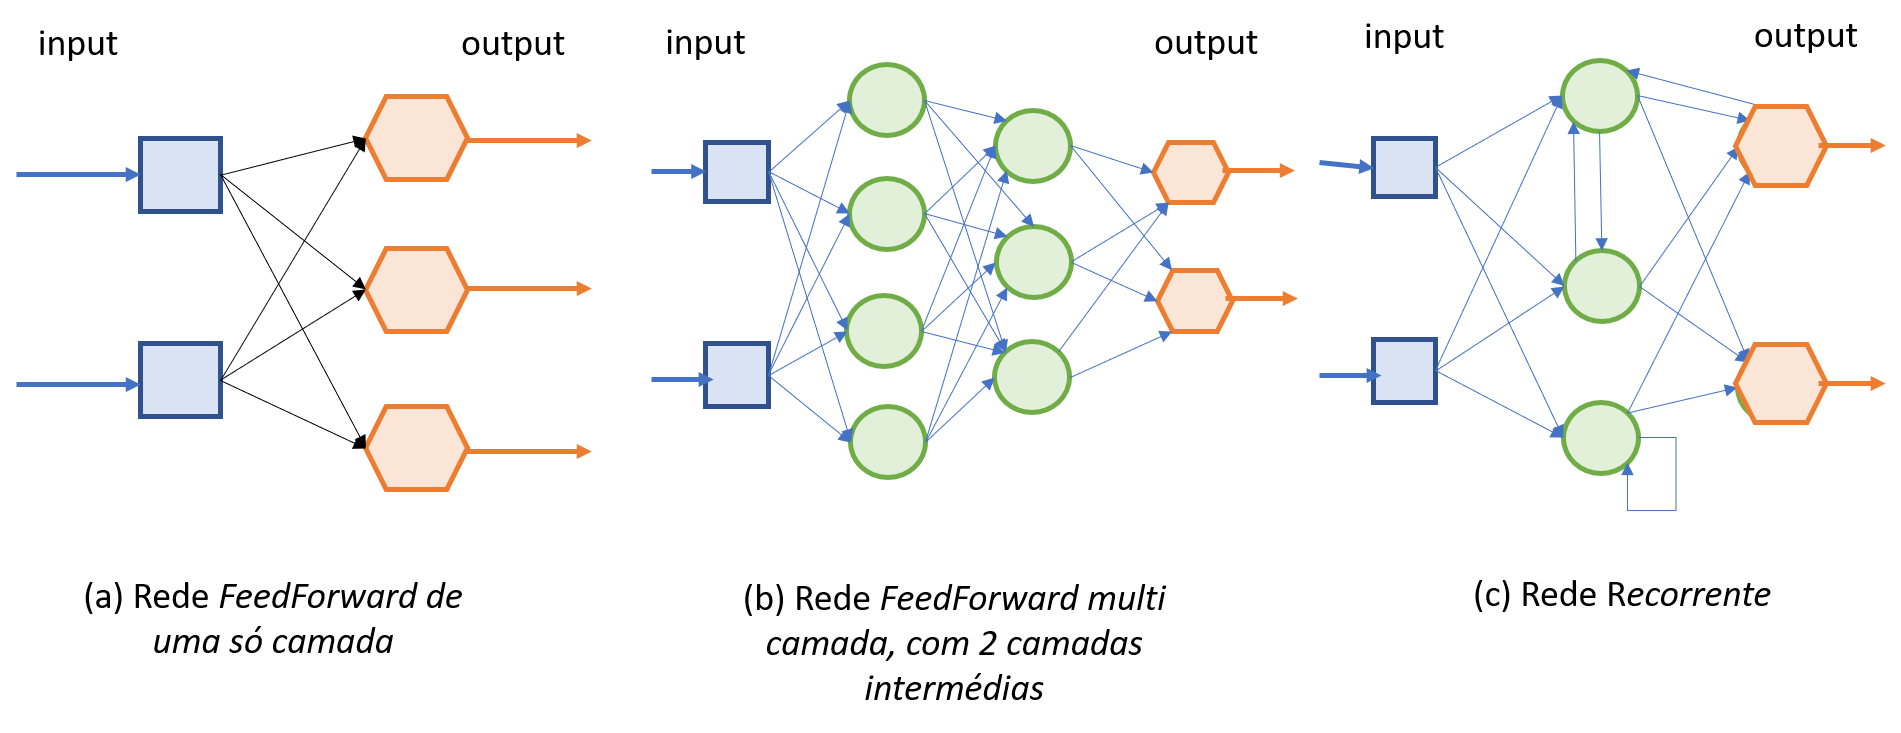
\includegraphics[scale=0.5]{Imagens/topos.png}
    \caption{Exemplos de algumas topologias de arquiteturas de RNAs}
    \label{fig:arquiteturas}
\end{figure}

\section{\textit{Back-Propagation}}
\label{sec:backProp}

Associado ao método de aprendizagem do Gradiente Descendente, o algoritmo de \textit{Back-Propagation} é um dos algoritmos mais utilizados no paradigma de aprendizagem supervisionada de redes neuronais artificiais. 

Regras de aprendizagem do tipo Gradiente Descendente baseiam-se na diminuição de um erro, sendo este estimado entre um valor pretendido e um valor obtido pela previsão da rede. \cite{Haykin-ANN}
Para cada estado do processo de evolução da rede, o objetivo prende-se com a minimização de uma função de custo, definida em termos do valor de erro. 

Este processo de avaliação é descrito pela Equação \ref{eq1}, onde $\eta$ é a taxa de aprendizagem e $\Delta \epsilon$ a diferenças entre o valor esperado e o valor obtido para uma dada entrada (gradiente da função de custo).  

\begin{equation}
    \label{eq1}
    \Delta w = \eta \Delta \epsilon
\end{equation}

No caso especifico do algoritmo de \textit{Back-Propagation}, a sua implementação segue os seguintes passos:
\begin{itemize}
    \item Antes de se iniciar o treino, são atribuídos valores aleatórios aos axónios da arquitetura, marcando assim o peso inicial de cada ligação; 
    
    \item Iniciado o treino, os valores (vetores entrada) fornecidos aos nodos de input  vão-se propagando para a frente, até chegarem aos nodos de saída. Chegando à camada final, é calculado o erro entre o valor obtido pela rede e o valor esperado; 
    
    \item O referido erro é propagado para as camadas anteriores, desde os nodos de saída até aos aos nodos da camada de \textit{input}. Esta retro propagação leva ao ajustamento dos pesos de cada nodo segundo a regra de \textit{Widrow-Hoff} Equação \ref{eq1};
    
    \item Este processo é repetido para cada iteração. A fase de treino termina quando forem cumpridos os critérios de paragem definidos.
\end{itemize}

\chapter{Análise Exploratória Dados}
\label{chp:AnaliseDados}

\section{\textit{Dataset} em estudo}
\label{sec:DatasetEstudo}

Como referido, neste projeto procura-se utilizar as capacidades de generalização de uma \textit{Rede Neuronal Artificial} para a identificação do nível emocional de uma determinada publicação, com base nas palavras utilizadas na sua composição.  

Como suporte de dados para o processo de treino e teste da rede, foi utilizado um \textit{dataset} com informações de publicações da rede social \textit{Twitter}, recolhidas num período entre 1 de janeiro de 2016 e 31 de Julho de 2017. 
Será sobre este conjunto de dados que recai a fase de pré processamento de dados, abordada ao longo deste capítulo.

Como principais atributos, o referido \textit{dataset} apresenta inicialmente os campos:

\begin{itemize}
    \item \textbf{\textit{UserLocation}} – (\textit{String}) Representação textual da localização do utilizador que realizou a publicação. 
    A localização toma a forma de uma string, geralmente com o nome da cidade e o país. Pode também apresentar apenas as coordenadas de longitude e latitude ou valores nulos;
    
    \item \textbf{\textit{IdPost}} – (\textit{Inteiro}) Identificador único de cada uma das publicações;
    
    \item \textbf{\textit{TextPost}} – (\textit{String}) Conteúdo textual da publicação. 
    Apresenta a informação relevante que se procura analisar, após pré tratamento e adaptação, com base em RNAs;
    
    \item \textbf{\textit{Hashtags}} – (\textit{String}) Conjunto de \textit{hashtags} utilizadas junto da publicação. 
    
    Num sentido de uniformização, no contexto do \textit{dataset} identifica-se por "\textit{hashtags}" o conjunto de palavras iniciadas pelo carácter $\#$ e que procuram identificar as palavras chave ou tópicos da publicação. 
    
    Este campo pode encontrar-se vazio (valores nulos) ou conter um conjunto de um ou mais \textit{hashtags};
    
    \item \textbf{\textit{Date}} – (\textit{Data}) Registo da data em que a publicação foi colocada online, segundo o formato "Dia/Mês/Ano Hora:Minutos". 
    
    Cerca de 279 instâncias contêm este atributo como nulo;
    
    \item \textbf{\textit{TweetLat}} – (\textit{Inteiro}) Valor da latitude na qual a publicação foi colocada online;
    \item \textbf{\textit{TweetLon}} – (\textit{Inteiro}) Valor da longitude na qual a publicação foi colocada online;
    
    \item \textbf{\textit{PhotoLat}} e \textbf{\textit{PhotoLon}} – (\textit{Inteiros}) Valores da latitude e longitude associados à fotografia colocada junto com a publicação.
\end{itemize}

No total, o \textit{\textit{dataset}} é composto por um conjunto de 990473 instâncias. Nas seguintes secções serão destacadas as alterações realizadas ao dataset a nível de limpeza e criação de novos atributos. 

\section{Análise dos atributos}
\label{sec:AnaliseAtributos}

No sentido de identificar o nível emocional de uma publicação, foi inicialmente realizado um estudo aos dados fornecidos, no sentido de interpretar os seus valores e determinar qual a relevância de cada um dos atributos neste contexto.

Nesta secção, procura-se assim justificar a escolha dos atributos do dataset a as alterações que se realizaram ao mesmo. 
Tal como já referido, o conjunto de dados recolhidos resulta da recolha de um conjunto de informações associadas a diversas publicações na rede social \textit{Twitter}. 

\begin{multicols}{2}
\begin{itemize}
    \item \textit{UserLocation}
    \item \textit{IdPost}
    \item \textit{TextPost}
    \item \textit{Hashtags}
    \item \textit{Date}
    \item \textit{TweetLat / TweetLon}
    \item \textit{PhotoLat / PhotoLon}
\end{itemize}
\end{multicols}

O primeiro processo de filtragem de qualidade destes parâmetros baseia-se na presença de valores nulos, ou seja, no número de registo em falta para um determinado atributo. 
Nesse sentido, os atributos \textit{TweetLat, TweetLon, PhotoLat} e \textit{PhotoLon} foram automaticamente removidos, por apresentarem uma taxa de valores nulos de 100\%. 
Sendo valores inteiros, esta informação foi conseguida através de uma análise segundo a ferramenta \textit{Weka} (Figura \ref{fig:analiseWeka}).  

\begin{figure}[t]
    \centering
    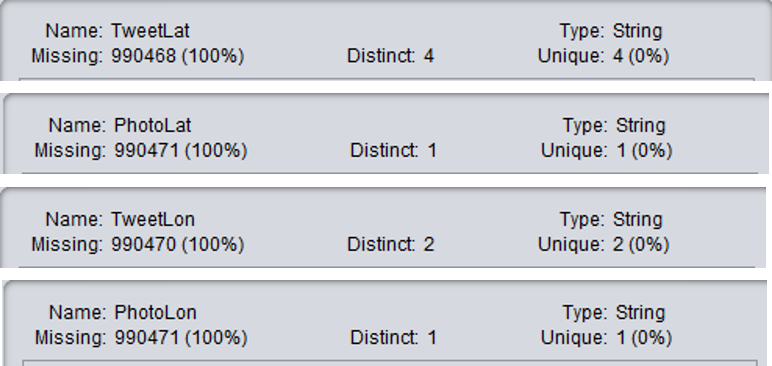
\includegraphics[scale=1]{Imagens/weka1.png}
    \caption{Análise do número de valores nulos e distintos dos atributos do dataset, recorrendo à ferramenta \textit{Weka}}
    \label{fig:analiseWeka}
\end{figure}

Sendo que por si só, a análise de linguagem natural já é um processo bastante dependente do contexto da frase e da forma como se organizam as palavras, uma das dificuldades associadas a este tipo de processamento recai na ambiguidade das palavras. 

Neste sentido, o uso de palavras soltas pode estar associado a diversos contextos emocionais ou até com formas de estilo como ironia. Por este motivo, foi tomada a decisão de ignorar quais \textit{hashtag} existente no dataset, dado que no contexto não apresentam um conhecimento sólido para o processo de aprendizagem da rede.

Assim, foi removida integralmente a coluna relativa ao atributo \textit{Hashtags}, que continha a listagem de eventuais \textit{hashtags} associados à publicação. 

O atributo \textit{IdPost} foi também removido nesta fase inicial de limpeza, dado que por ser único para cada publicação, não apresenta qualquer informação capaz de ser apreendida e generalizada pelo processo de aprendizagem da rede neuronal artificial. 

Os parâmetros \textit{UserLocation} e \textit{Date} foram mantidos por apresentarem alguma integridade nos seus valores. 
Numa fase posterior ao treino e teste de desempenho da RNA, estes registos podem eventualmente ser utilizados para gerar dados e estatísticas com base na localização do utilizador e o nível emocional da publicação. Contudo, não serão utilizados nem adaptados para o processo de treino da rede. 

Em suma, de todos os atributos do conjunto de dados, aquele que será exclusivamente adaptado para ser utilizado no processo de evolução da rede será o conteúdo textual da publicação, \textit{TextPost}, dado que é sobre este texto que se procura classificar o nível emocional da frase.

\section{Adaptação do \textit{Dataset}}
\label{sec:AdaptacaoDataset}

Como referido na secção anterior, a análise da semântica de um determinado texto está intrinsecamente ligado com o contexto em que a frase é composta e de que forma as palavras estão organizadas na mesma. 

Para um processo de análise de texto com base em algoritmos de \textit{Machine Learning}, registos com palavras soltas como os \textit{hashtags} ou hiperligações para páginas online, são alguns dos exemplos de informações que não apresentam nenhum material útil para o processo de extração de conhecimento. 

Relativamente a estes dois tipos de "palavras":
\begin{itemize}
    \item Analisar um \textit{hashtag} pelo valor da palavra em si, seria assumir de forma implícita um contexto para essa palavra e utilizar o peso da palavra nesse contexto em qualquer publicação onde esse \textit{hashtah} fosse utilizado.
    
    A titulo de exemplo, uma publicação com um contexto negativo e associado a tristeza pode apresentar um hashtag com a palavra \textit{"happy"}, meramente aplicada num contexto de ironia e como tal, oposta ao verdadeiro sentido emocional da publicação.
    
    Neste sentido, atribuir valor às palavras individuais dos \textit{hashtags} seria afetar o desempenho de classificação e enviesar a capacidade de análise de qualquer processo de aprendizagem que fosse utilizado. 
    
    Por este motivo, foram também removidos todos os \textit{hashtags} que surgissem no conteúdo textual da publicação. 
    Para isso foi simplesmente utilizada a ferramenta \textit{NotePad++} e utilizada a expressão regular \textit{\#( [a-zA-Z0-9] | [À-ÿ] )*} para apanhar todos os \textit{hashtags}. 
    
    \item Apesar de ser possível, a partir do endereço de uma hiperligação, utilizar uma API para extrair todas as palavras-chave associadas ao conteúdo dessa página, a obtenção desta lista de palavras-chave levaria ao mesmo problema que os \textit{hashtags}, descrito no tópico anterior. 
    
    Como consequência, todas as referências a hiperligações foram também removidas do conteúdo do texto da publicação. 
    
    Contudo, a representação de \textit{urls} estava bastante fragmentada e incoerente, tendo mostrado alguma dificuldade numa completa limpeza dos mesmos. A solução passou pelo uso de expressões regulares mais complexas, criadas para o contexto e,  uso dos métodos do \textit{package Tweet PreProcessor} existentes em \textit{Python}. 
    
\end{itemize}

Focando no conteúdo da publicação que é efetivamente útil para análise, é relevante frisar que no \textit{dataset} fornecido não existe qualquer relação entre as frases das publicações e o valor emocional associado às mesmas. 

Dado que este projeto recai sobre o uso de RNAs segundo um paradigma de aprendizagem supervisionado, é necessário fornecer à rede um conjunto de dados de treino junto com o respetivo conjunto de \textit{labels}, que identifique qual o resultado de \textit{output} esperado para um cada \textit{input} de treino.

Para gerar estas informações é necessário recorrer àquilo que pode ser visto como um dicionário, que mapeia o valor de uma palavra com o nível de sentimento a si associado. 
Analogamente, a forma mais simples de medir o peso emocional de uma frase, recai também no uso destas estruturas, somando o peso das palavras que compõe uma frase.  

Para gerar esta métrica para cada uma das instâncias do dataset, foram tidas em conta as seguintes considerações: 

\begin{itemize}
    \item O dataset é composto por publicações em diversas linguagens, nomeadamente inglês, francês e italiano;
    
    \item Utilizar as instâncias apenas com publicações em inglês seria reduzir significativamente o volume do \textit{dataset} e, com isso, perder informação relevante para o processo de aprendizagem da rede; 
    
    \item Não sendo viável remover todas as publicações que não se encontrem em inglês e dado que a maioria dos dicionários <Palavra, Valor-Emocional> existentes e disponíveis recaem na terminologia inglesa, uma das soluções passa pela tradução de todos as instâncias para a inglês. 
    
    Contudo, recorrendo à API de tradução disponibilizada pela plataforma \textit{Google Translate} \cite{googleTransAPI}, o processo de tradução é implementado sobre pedidos http. 
    Cada pedido envolve o encapsulamento (\textit{marshling e unmarsheling}) de pacotes \textit{JSON} com o conteúdo e resposta da tradução, pelo que o tempo de cada tradução andava acima de 1 segundo por frase/publicação. 
    
    Dado o tempo disponível para este projeto e a dimensão do dataset (+ de 900 mil instâncias), a opção de traduzir cada publicação não se apresenta viável;
\end{itemize}

A solução encontrada passou pelo uso de uma nova API de mapeamento <Palavra, Valor-Emocional> que fosse capaz de lidar com várias linguagens, evitando assim que fosse necessária uma tradução prévia do conjunto de dados. 

É com base neste nível de sentimento, quantificado num valor numérico, que se mapeia o peso emocional das frases de uma publicação numa das seguintes classes:

\begin{multicols}{3}
\begin{itemize}
    \item \textit{Negativo}
    \item \textit{Neutro}
    \item \textit{Positivo}
\end{itemize}
\end{multicols}

Apesar do enunciado do projeto especificar que as classes de classificação da RNA deveriam ser apenas $"\textit{Negativo}"$ ou $"\textit{Positivo}"$, foi tomada a decisão que a classificação seria mais coerente e rigorosa de existisse também o nível \textit{Neutro}.

Desta forma, a \textit{tag} $"Neutro"$ procura representar as publicações que não apresentam qualquer nível sentimental, seja porque o seu conteúdo é ambíguo de interpretar ou porque são frases simples, que procuram apenas descrever factos ou eventos. 

Pelo facto de uma frase não ser simplesmente positiva ou negativa, justifica-se assim a decisão de existirem 3 classes de previsão. 


\section{Criação de Atributos \textit{Target/Output}}
\label{sec:CriacaoTarget}

Para a criação deste novo atributo, que representa o output sobre o qual a rede deve treinar e ser capaz de realizar previsão, foram exploradas algumas soluções de análise de texto já implementadas na linguagem \textit{Python}. 

Relativamente à escolha de uma API capaz de realizar uma análise em linguagem natural e deteção de sentimentos, foram exploradas as seguintes soluções:

\begin{itemize}
    \item \textbf{\textit{Natural Language Toolkit - NLTK}} \cite{NLTK}: A plataforma \textit{NLTK} apresenta-se como uma das ferramentas \textit{Open-source} mais utilizadas para desenvolver algoritmos ou métodos que necessitem de analisar linguagem humana num contexto semântico. 
    
    No contexto de análise de sentimentos em frases, os métodos desta ferramenta baseiam-se em técnicas de Classificação hierárquica para determinar o nível de polaridade e subjetividade de uma frase. Por polaridade entende-se o nível de sentimento de uma frase (positivo ou negativo) e por subjetividade entende-se o nível de confiança da classificação, conforme o contexto e conteúdo da frase analisada. 
    
    A \textit{API} desenvolvida para \textit{Python} \cite{NLTK-python} apresenta como pontos positivos e facto de devolver a Polaridade dividida em dois valores decimais, para identificar a percentagem de sentimento negativo ou positivo na frase. 
    
    Contudo, o seu foco encontra-se ainda muito voltado para a língua inglesa, tornando-a assim inadequada para o dataset em análise, pelos motivos supracitados na listagem anterior. 
    
    \item \textit{\textbf{Microsoft Azure: Text Analytics AP}} \cite{azure}: Disponibilizados na plataforma \textit{Azure}, a Microsoft disponibiliza um conjunto de soluções que designa como "Serviços cognitivos" pela sua envolvência com a temática da inteligência artificial. 
    
    Estes serviços oferecem APIs para processamento de imagem, voz, conhecimento e linguagem. É nesta ultima área que surge a ferramenta \textit{Text Analytics} \cite{azureAPI}.
    
    Esta solução é capaz de, para uma determinada entrada de texto, automaticamente determinar a sua linguagem e devolver o seu nível de sentimento, junto com uma lista de palavras chave/\textit{target} que permitem atribuir um determinado nível de sentimento à frase. 
    
    Apesar da ferramenta funcionar com um grande número de linguagens e apresentar uma elevada capacidade de análise para frases com palavras relacionadas entre si, a chave de utilização deste serviço é limitada a 30 dias e a 5000 pedidos por dia. 
    
    Novamente, a exploração integral do dataset com esta API seria impossível, devido ao seu volume de dados e ao domínio temporal deste projeto. 
    
    \item \textit{\textbf{TextBlob}} \cite{textblob}: Procurando contornar as limitações encontradas nas duas ferramentas anteriores, a biblioteca \textit{TextBlob} apresenta-se como a solução encontrada para pré processar o dataset limpo, como forma de calcular o nível de sentimento de cada frase. 
    
    Esta plataforma é construida sobre a ferramenta \textit{NLTK} referida no primeiro ponto, embora acrescente sobre os seus métodos a capacidade de deteção de sentimentos em texto em várias linguagens nativas. 
    
    Por este motivo e, sendo totalmente \textit{open-source} e sem limite de pedidos, esta solução foi a utilizada para calcular os valores de sentimento de cada frase, sobre os quais a rede deve treinar e aprender a classificar/prever futuras frases de publicações. 

\end{itemize}

O uso da ferramenta \textit{TextBlob} envolve assim a tradução de publicações num idioma estrangeiro para inglês nativo, realizando uma tradução estocástica \cite{RepresentacaoTexto}. 

Considerando assim os resultados devolvidos pelos métodos da API \textit{TextBlob} para \textit{Python}, foram então acrescentadas duas colunas ao dataset:
\begin{itemize}
    \item A coluna \textbf{Polaridade}, que indica o nível de sentimento de um texto. 
        
    Toma valores decimais entre [-1, 1], sendo que frases com valores de polaridade próximos de -1 apresentam um conteúdo negativo e frases com valores de polaridade próximos de 1, associam-se a sentimentos positivos. 
        
    \item A coluna \textbf{Subjetividade}, onde se quantifica a confiança do nível calculado para o texto, conforme o seu contexto. 
        
    Toma valores decimais entre [0,1], sendo que valores próximos de 0 estão associados a textos bastante objetivos -nível de sentimento concreto para o contexto- e valores próximos de 1, recaem sobre textos subjetivos,onde a medição do nível de sentimento não é concreta para o contexto.
\end{itemize}

Relembrando que se procura classificar o nível emocional de uma frase apenas em três classes concretas (Secção \ref{sec:AdaptacaoDataset}), é necessário realizar uma descriterização dos valores tomados pelo atributo Polaridade. 
Uma vez que a API fornece duas métricas relevantes, foi tomada a decisão de conjugar estas duas informações num único atributo, que mapeia os valores dentes os parâmetros Polaridade e Subjetividade para uma das classes objetivo: Negativo, Neutro ou Positivo.  

Como forma de não criar tendências no processo de aprendizagem, nem classificar como positiva ou negativa frases com conteúdo/contexto ambíguo, foi tomada a decisão que todas as instâncias com subjetividade superior a 0.5 representam publicações com um conteúdo neutro. 

Para os restantes casos, onde exista pelo menos 50\% de certezas face à objetividade da publicação e ao seu contexto, o mapeamento do valor da polaridade para uma das três classes referidas foi realizado dividindo o intervalo de valores deste atributo de forma linear. 
A figura \ref{fig:niveisSentimento} procura descrever esquematicamente esta divisão. 

\begin{figure}[t]
    \centering
    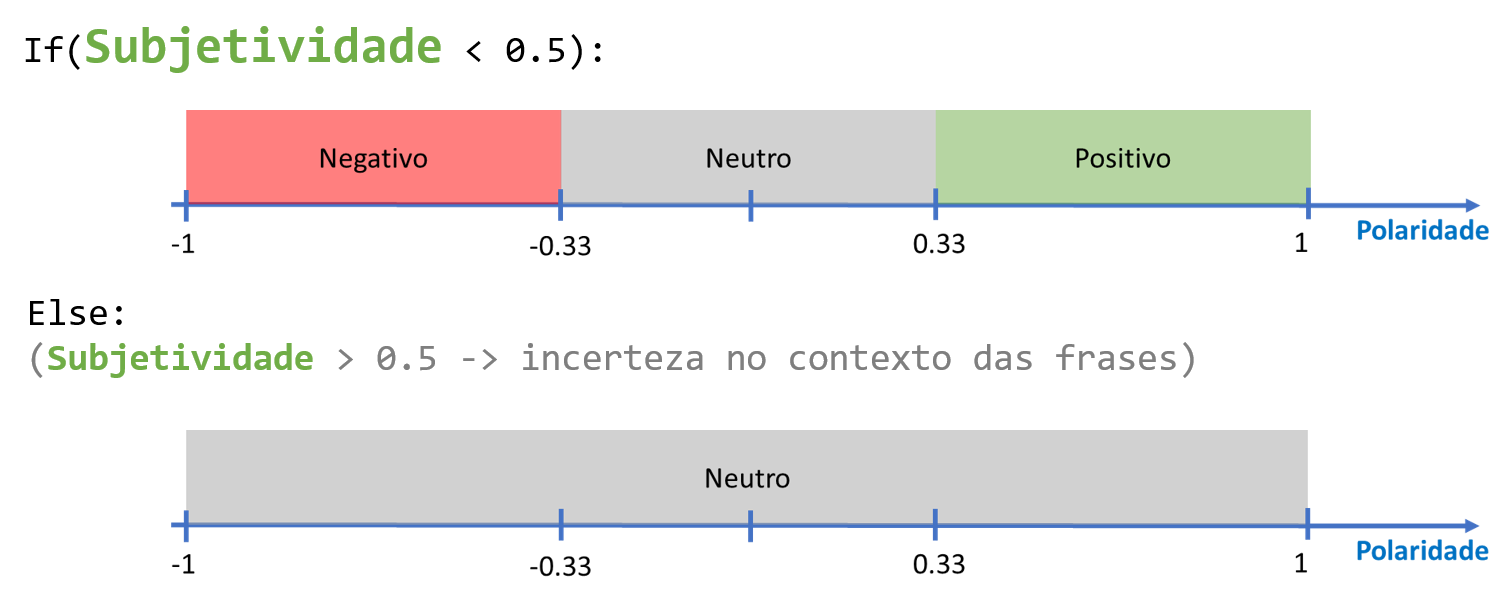
\includegraphics[scale=0.5]{Imagens/niveisSentimento.png}
    \caption{Mapeamento dos valores de polaridade e subjetividade para as classes "Negativo", "Neutro" e "Positivo". }
    \label{fig:niveisSentimento}
\end{figure}

Conjugando os resultados da API \textit{TextBlob} com o mapeamento acima referido, foi possível observar que uma massiva maioria dos casos foi identificada apenas com um valor neutro de sentimentos. (Figura \ref{fig:medidas})
Apenas cerca de 8\% das instâncias do dataset foram identificadas como associadas a um sentimento negativo/positivo. 

Sendo que as outras APIs de classificação textual, possíveis de utilizar para criar o atributo \textit{target}, se baseiam nos mesmo processos de classificação de linguagem natural, conclui-se que o dataset pode não ser o melhor para treinar de forma viável uma RNA, devido à discrepância entre casos neutros com os casos associados a sentimentos negativos/positivos. 

\begin{figure}
    \centering
    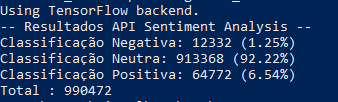
\includegraphics{Imagens/medidas.png}
    \caption{Percentagens de publicações classificadas num determinado nível de sentimento: Negativo, Neutro ou Positivo. }
    \label{fig:medidas}
\end{figure}

\section{Redução Dataset}
\label{sec:reducaodataset}

Tendo sido observado que o volume inicial do dataset se apresentaria como uma entrave para a construção de RNAs mais complexas e de maiores dimensões, foi tomada a decisão de reduzir significativamente o número de casos utilizados no processo de aprendizagem da rede. 

Uma vez que a manipulação do conjunto de dados completo implicaria recursos de memória e tempo de processamento não disponíveis no decorrer deste projeto, foram assim criadas a partir dele cerca de 100 mil instâncias para Treino e Teste das RNAs. 
Este novo dataset, apesar de conter cerca de $\frac{1}{10}$ do volume inicial, apresenta ainda assim uma quantidade significativa de casos, filtradas com mais detalhe e rigor a nível de tradução para a língua inglesa. 

Neste conjunto de dados foram selecionados 100 mil casos aleatórios do dataset inicial. 
Como pré processamento adicional, foi dado ênfase à limpeza de palavras com caracteres desconhecidos e referências a conteúdos sem informação útil para o processo de aprendizagem. 
Além disso, foi ainda utilizada a API do \textit{Google Translator} para realizar a tarefa de tradução cuidada dos \textit{tweets}. (No dataset completo não foi possível usar esta ferramenta devido ao tempo de tradução do dataset inteiro)

Esta redução permite aumentar a complexidade da rede, a nível de camadas intermédias e número de \textit{Epochs}, levando à possibilidade de mais cenários de treino/teste de RNAs. 
Ao utilizar-se um dataset de menores dimensões, o tempo de aprendizagem da rede e recursos necessários para representar os \textit{tweets} do dataset em formato de input da rede são significativamente menores.

\chapter{Desenvolvimento da RNA}
\label{chp:criacaoRNAs}

Uma vez que a fase de pré processamento do dataset foi implementada com funções auxiliares desenvolvidas em \textit{Python}, para a frase de desenvolvimento da RNA manteve-se a mesma linguagem de programação. Assim, alem de se manter o mesmo ambiente de desenvolvimento, \textit{Python} disponibiliza as principais APIs de criação de RNAs atualmente utilizadas. 

Como plataforma escolhida para executar a rede, foi utilizada a ferramenta \textit{Keras}. 
Esta ferramenta apresenta um conjunto de características que se adequam com o contexto deste projeto, nomeadamente: 
\begin{itemize}
    \item É bastante simples de usar, permitindo rapidamente obter uma estrutura de rede capaz de analisar os dados. 
    
    Contudo, permite também evoluir a rede a nível de complexidade, interligando com outras plataformas de criação de RNAs (\textit{TensorFlow, Theano, CNTK}) e permitindo ainda alterar o contexto de execução da RNA (CPU ou GPU);
    
    \item Devido ao volume do dataset apresentar mais de 900 mil instâncias, alimentar a rede com todos os dados numa fase de treino única exigia recursos e uma capacidade de processamento continua durante demasiado tempo. 
    
    Contudo, os métodos da plataforma \textit{Keras} permitem criar várias fases de treino, que evoluem a rede face ao estado de treino anterior. Desta forma é possível dividir o dataset em subconjuntos que são utilizados em fases de treino iterativas, exigindo assim menores recursos de memória e tempo de processamento na fase de aprendizagem;
    
    \item Pelo mesmo motivo do tópico anterior, treinar a rede sempre que for necessário realizar algum tipo de previsão não é viável em problemas com um elevado número de dados. 
    
    Como solução, \textit{Keras} disponibiliza funções para guardar o estado da RNA. É assim possível armazenar tanto a arquitetura, como os pesos das ligações dos axónios, após uma fase de treino ou teste da rede;
    
    \item \textit{Keras} permite parametrizar praticamente todos os aspetos relacionados com a topologia da rede, como o número de camadas; ligações entre camadas; funções de ativação por camada; métricas de avaliação interna da rede e o \textit{optimizer} (método de aprendizagem da rede). 
\end{itemize}

Tendo por base a experiência anterior com outras plataformas de desenvolvimento de RNAs, como \textit{R, Julia ou MXNet}, a plataforma \textit{Keras} apresenta-se como a mais indicada e modular para este contexto.
Focando o conjunto de motivos anterior e sendo atualmente uma plataforma bastante utilizada para a criação de RNAs, a plataforma \textit{Keras} foi assim a escolhida para o desenvolvimento da rede deste projeto. 


\section{Representação Texto \textit{Input} - Matrizes One-Hot}
\label{sec:vectPalavras}

Uma das decisões essenciais do uso de RNAs num problema de classificação de texto, passa por codificar as palavras/frases que compõe o texto num formato que seja capaz de ser analisado e processado corretamente pelos neurónios da rede. 

Devido à natureza da sua implementação, como o caso das funções de ativação que a rede utiliza na fase de aprendizagem, a sua estrutura está preparada para lidar apenas e preferencialmente com dados numéricos. Desta forma, uma palavra no seu formato literal e digital (\textit{Strings}) não são assim formatos indicados para alimentar e treinar uma rede que se procure treinar de forma viável e adequadamente. 

É assim necessário converter as palavras e a estrutura sequencial de uma frase num atributo (ou vários) caracterizado por valores numéricos. 
Encontrar formas de representação/tradução de linguagem natural para modelos de representação úteis em inteligência artificial não se apresenta como uma decisão simples, variando conforme o contexto sobre o qual se procura analisar a frase. 

Os dois procedimentos mais utilizados para representar texto são associados com as estruturas \textit{Vector Embeddings} ou Matrizes \textit{One-Hot}. 
\textit{Embeddings Vectors} são mapeamentos no espaço de palavras e/ou frases, em que a sua localização indica as semelhanças (Figura \ref{fig:vectorEmbeddings}). Esta representação permite ainda associar relações semânticas, através da distancia dos vetores, sendo por isso muito usadas em contextos que envolvem a geração de analogias.

\begin{figure}[H]
    \hspace{-0.2in}
    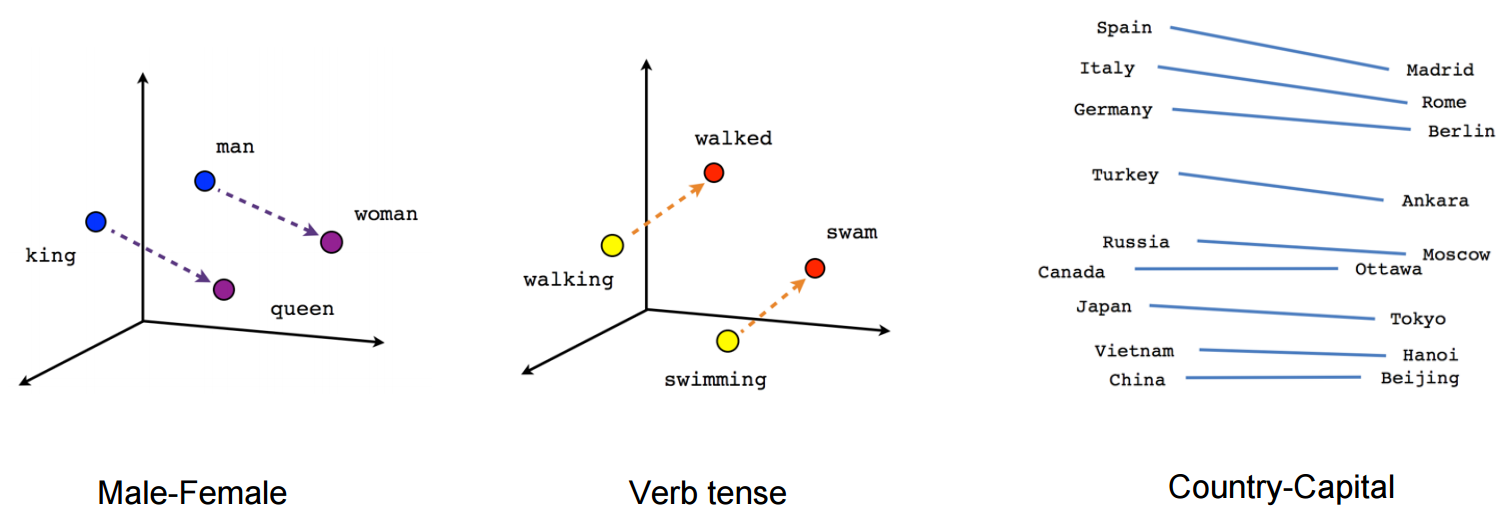
\includegraphics[scale=0.3]{Imagens/vector_embeddings.png}
    \caption{Representação simbólica de \textit{Vector Embeddings}}
    \label{fig:vectorEmbeddings}
\end{figure}


Em oposição, as estruturas matriciais \textit{One-Hot} não contêm informação de relações linguísticas entre as palavras. 
De uma forma geral, permitem apenas saber quais as palavras que surgem num determinado texto, não contendo informações sobre as relações entre as palavras, como a sua ordem ou semelhança na frase.

Para o contexto de classificação emotiva de texto, procura-se exatamente representar as palavras que se encontrem num determinado texto, num formato capaz de ser processado pelas camada de input de uma RNA. Nesse sentido, devido à sua simplicidade, as matrizes One-Hot foram o modelo de representação escolhido. 

Este tipo de matrizes são chamadas de \textit{One-Hot} já que cada matriz tem uma característica distinta ("hot") de todas as outras.

Considerando como exemplos as seguintes frases:
\begin{minted}[tabsize=4, breaklines=true]{text}
            Errors should never pass silently.
            Unless explicitly silenced.
\end{minted}

A representação numa matriz One-Hot das seguintes frases começa por "partir" as frases numa lista (vetor) de palavras, sem ocorrência de repetições. 

\begin{minted}[tabsize=4,breaklines=true]{Python}
    ['errors', 'should', 'never', 'pass', 'silently', 'unless', 'explicitly', 'silenced']
\end{minted}

Depois de criada a lista de palavras únicas no texto a representar, é criado aquilo que pode ser visto como um dicionário com todas as palavras distintas, atribuindo um id único a cada palavra. Neste processo, não é relevante a ordem das palavras. Cada id será apenas um identificador único de cada palavras e irá representar apenas o índice \textit{i,j} da matriz que representa aquela palavra.

\begin{minted}[tabsize=4,breaklines]{Python}
    {
          'errors': 0,      
          'should': 1,
          'never': 2,
          'pass': 3,
          'silently': 4,
          'unless': 5,
          'explicitly': 6,
          'silenced': 7,
    }
\end{minted}

Distribuídos os ids pelas palavras encontradas, a matriz \textit{One-Hot} terá tantas colunas quantas palavras encontradas no texto (dimensão dicionário) e, tantas linhas quantas as palavras encontradas na frase a codificar. 
No exemplo anterior, o dicionário de dados apresenta 8 palavras distintas e a primeira frase 5 palavras. Assim, uma matriz One-Hot que represente esta primeira frase terá dimensões 5x8. 

Em cada linha, o valor 1 no indice i,j que representa a palavra indica a ocorrência da mesma na palavra. Em oposição, o valor 0 indica a não ocorrência da palavra identificada pela linha. 

Para construir estas matrizes foram usados métodos disponibilizados na API \textit{Pre Processing Text} da plataforma \textit{Keras}. Nestas funções, as matrizes One-Hot devolvidas apresentam a vantagem de serem matrizes quadradas, podendo ser facilmente convertidas num vetor de palavras, considenrado apenas os valores da sua diagonal. Deste modo, o valor 1 num determinado indice indica a ocorrência, ou não, daquela palavra no texto representado pelo vetor de palavras. 

\begin{minted}[tabsize=4,breaklines]{Python}
    [
        [1, 0, 0, 0, 0, 0, 0, 0], #errors
        [0, 1, 0, 0, 0, 0, 0, 0], #should
        [0, 0, 1, 0, 0, 0, 0, 0], #never
        [0, 0, 0, 1, 0, 0, 0, 0], #pass
        [0, 0, 0, 0, 1, 0, 0, 0], #silently
        [0, 0, 0, 0, 0, 0, 0, 0], #unless
        [0, 0, 0, 0, 0, 0, 0, 0], #explicitly
        [0, 0, 0, 0, 0, 0, 0, 0], #silenced
    ]
\end{minted}

Na implementação utilizada, utilizaram-se vetores de palavras com 3500 posições, representando assim a 3500 palavras mais utilizadas. 
Infelizmente, apesar desta representação ser bastante simples e eficaz no contexto, implica que as RNAs apresentem tantos nodos de \textit{input} quantos índices do vetor. 

Por este motivo e por questões de memória, para representar em vetores de palavras todos os tweets utilizados na fase de aprendizagem da rede, foram apenas utilizados vetores com 3500 posições. 

\section{Arquitetura da RNA}

Para a definição da topologia da rede neuronal, foi utilizada uma arquitetura multi-layer FeedForward (Secção \ref{sec:Arquiteturas}). Em \textit{Keras} este tipo de rede designa-se como \textit{sequencial} e representa assim uma rede \textit{multi-layer perception}.

A criação de diferentes camadas camadas intermédias recorre ao método \textit{Dense}, que na plataforma caracteriza uma camada de neurónios totalmente conectada com os neurónios da camada anterior. 

\begin{minted}[tabsize=4, breaklines=true]{Python} 
    # Exemplo da Definicao da topologia da rede
    self.model = Sequential()
    self.model.add(Dense(512, input_shape=(self.max_words,), activation='tanh', kernel_initializer="uniform"))
    self.model.add(Dropout(0.5))
    self.model.add(Dense(256, activation='tanh', kernel_initializer="uniform"))
    self.model.add(Dense(128, activation='tanh', kernel_initializer="uniform"))
    self.model.add(Dense(3, activation='tanh'))
\end{minted}

Neste processo de criação de diferentes topologias foram tido alguns cuidados, destacando-se os seguintes aspetos: 

\begin{itemize}
    \item Na primeira camada intermédia, através do parâmetro \textbf{\textit{input\_shape}} a camada identifica automaticamente o número de neurónios da camada de input. 
    Neste caso, existem tantos neurónios de input quantos elementos do vetor de palavras que representa a frase do \textit{Tweet} (Secção \ref{sec:vectPalavras});
    
    \item O argumento \textbf{\textit{activation}} define a função de ativação a utilizar na camada. 

    Muitas das principais funções utilizadas em contextos de RNAs apresentam apenas um contradomínio entre [0,1] ou [0, inf].
    Uma vez que existem três classes target ({Negativo, Neutro, Positivo}), identificadas respetivamente pelos valores {-1, 0, 1}, foi tido o cuidado de utilizar funções de ativação que mantivessem o seu contradomínio entre [-1, 1]. 
    
    Utilizar funções sem contradomínio negativo, reduziria a capacidade de aprendizagem dos casos de publicações com nível emocional negativo. 
    Contudo, como em teoria o processo de aprendizagem é capaz de lidar com nodos que sejam reduzidos ao valor 0, foram também utilizadas algumas funções com contradomínio diferente de [-1, 1]. 
    
    Nomeadamente, foram experimentadas algumas adaptações da função ReLU;
    
    \item O parâmetro \textbf{\textit{Kernel initializer}} define qual o método utilizado para gerar o valor inicial dos pesos das ligações. 
    
    Neste projeto foram exploradas funções como a distribuição normal, uniforme e, maioritariamente, a distribuição de \textit{Xavier} \cite{xavier}.
    
    \item Na tentativa de evitar cenários de overfitting, podem ser adicionadas camadas \textit{Dropout} através de um método com o mesmo nome.
    
    \begin{minted}[tabsize=4, breaklines=true]{Python} 
        # Exemplo da adição de uma dropout layer com probabilidade = 0.2
        self.model.add(Dropout(0.2))
    \end{minted}
    
    O processo de \textit{dropout} acontece apenas na fase de treino e ocorre depois da fase de ativação do neurónio. 
    Esta camada opera de forma aleatória, colocando algumas ativações com o valor zero. Desta forma é simulado o conceito de "esquecimento", descartando alguma informação e "apagando" partes da rede neuronal em algumas iterações. 

    Contudo, estas camadas não devem ser introduzidas logo na fase inicial e foram exploradas apenas em cenários de overfitting ou na tentativa de obter melhores resultados de classificação. 
\end{itemize}

\section{Padrões de Treino}
\label{sec:padroesTreino}

Depois de especificada a arquitetura que dará suporte à representação da rede neuronal, o processo de aprendizagem da rede pode ser dividido em duas etapas: a definição de uma método de aprendizagem, segundo um conjunto de métricas de avaliação e, a fase de análise e generalização efetiva dos dados, realizando o ajustamento dos pesos da rede aos mesmos. 

\subsection{Método de Aprendizagem}

Para definir o comportamento de aprendizagem da rede é utilizado o método \textit{Compile}. 

Na escolha de um optimizador e métricas de avaliação, necessários de fornecer a este método, foram tomadas as seguintes considerações:
\begin{itemize}

    \item O parâmetro \textit{optimizer} define a técnica de aprendizagem utilizada. Neste projeto foi escolhido o método Adam \cite{adam2}. 
    
    Este algoritmo, além de atingir bons resultados de forma rápida, apresenta ainda benefícios dos métodos AdaGrad (Gradiente descendente adaptativo) e RMSProp (\textit{Root Mean Square Propagation}) \cite{adam1}.
    
    Uma vez que o método já está incluído dentro do \textit{Keras}, basta fazer referência ao seu nome. Por omissão são utilizados os parâmetros aconselhados no artigo em que a técnica foi apresentada.
    
    \begin{minted}[tabsize=4, breaklines=true]{Python} 
        Keras.optimizers.Adam(lr=0.001, beta_1=0.9, beta_2=0.999, epsilon=None, decay=0.0, amsgrad=False)
    \end{minted};
    
    \item O parâmetros \textit{loss} define a técnica de avaliação de desempenho da rede, através de uma função objetivo que o modelo da RNA irá minimizar.
    
    Apesar de várias implementações se basearem na métrica \textit{Binary Cross Entropy}, esta adequa-se apenas a cenários com apenas 2 classes de previsão. Como foi assumido que neste projeto a RNA será capaz de classificar três níveis de emoção, terá que ser utilizado o método \textit{Categórico};
    
    Por se tratar de um problema de classificação, foram exploradas as opções \textit{Mean Squared Error (MSE)} e \textit{Categorical Cross Entropy} para este parâmetro.
        
    \item O último parâmetro indica uma lista de métricas a utilizar para avaliar a capacidade de previsão/classificação da rede. 
    
    Neste processo de treino, por se tratar de um problema de classificação, foi mantida a métrica \textit{Accuracy}. 
    
\end{itemize}

O seguinte excerto de pseudo código procura descrever a definição do método de aprendizagem dentro da plataforma \textit{Keras}.

\begin{minted}[tabsize=4, breaklines=true]{Python} 
    # Definição arquitetura e topologia
    model = Sequential()
    # model.add( ... )
    # (...)
    
    # Definição processo aprendizagem RNA
    model.compile(optimizer='adam', loss='categorical_crossentropy', metrics=['accuracy', 'mse'])
\end{minted}

\subsection{Parâmetros Treino Rede}
\label{sec:ParametrostreinoRede}

Para o treino da rede, é utilizada a função \textit{fit}, que permite realizar o treino da rede num determinado contexto de execução.

Relativamente ao processo de treino, foram tomadas as seguintes considerações ao longo das sucessivas experiência de treino: 

\begin{itemize}
    \item O parâmetro \textit{Epochs} define o número de passagens completas pelos dados, na fase de treino da RNA. 
    O processo em que todas as instâncias de um dataset avança para a frente (\textit{forward} propagation) na rede, até aos nodos de output e novamente para trás (\textit{backward} propagation), até aos nodos de input, define assim um \textit{Epoch}. 
    
    Nos contextos em que uma rede treine sobre um dataset de pequenas dimensões, justifica-se que se explorarem valores de \textit{Epochs} elevados, dado que atualizar os pesos das ligações apenas com poucas passagens pelos dados pode não ser suficiente. 
    
    Se por um lado um baixo número de \textit{Epochs} pode levar a \textit{underfitting} da capacidade de aprendizagem da rede, valores elevados pode levar a tendências de \textit{overfitting} aos dados. 
    
    Como neste cenário o dataset apresenta uma grande volume de dados (perto de 1 milhão de linhas/ cerca de 600 mil para treino da RNA), o dataset contem por si só imensos exemplos diversificados de publicações. 
    Por este motivo, o número de passagens pelos dados foi explorado apenas com valores baixos, como 10, 12, 15, 20 ou 25.  
    
    Valores de Epochs superiores a 25 aliados a \textit{Batchs} de pequenas dimensões, fazem crescer exponencialmente o tempo de treino da rede. 
    
    \item o parâmetro \textit{Batch\_size} controla o número de exemplos presente num \textit{Batch}. 
    
    Apesar do dataset ser externamente dividido e processado em fases de treino iterativas, um subconjunto do dataset não pode ser passado integralmente à rede para treino. Assim, este parâmetro controla o número de instâncias que são alimentadas à rede em cada iteração de uma fase de treino.
    
    \textit{Batch sizes} de maiores dimensões permitem que mais dados sejam processados em simultâneo, reduzindo o tempo de execução da fase de treino. 
    Contudo, aumentar este parâmetro existe também uma maior quantidade de memória a cada iteração de treino da RNA. 
    
    Dado que neste projeto os dados de imput são vetores inteiros com pelo menos 3500 índices (Secção \ref{sec:vectPalavras}), este parâmetro foi explorado apenas com os valores {50, 100, 150, 250, 500}.
    
    Colocar valores mais pequenos não são viáveis, devido ao impacto que causa a nível do tempo de execução.  
    Mesmo o uso de 50 ou 100 exemplos por iteração, para RNAs com arquiteturas mais complexas, não se tornou viável de executar devido a limitações de memória, recursos de processamento e tempo necessários.
    (Treinar uma RNA durante dias não se adequa ao espectro de resultados esperados neste projeto simples).
    
    Em contrapartida, o uso de valores demasiado elevados, como 1000 ou 10000, leva a fases de treino que terminem de forma muito rápida mas precoce, sem permitir que a rede generalize adequadamente os dados que analisa.
    
    \item O parâmetro \textit{validation\_split} permite indicar qual a percentagem de dados do conjunto de treino que devem ser reservados para teste do processo de aprendizagem. 
    Como neste projeto o processo de treino é dividido em várias fases iterativas, devido às dimensões do dataset, não faz sentido criar avaliações de previsão em cada fase de treino. 
    
    Assim, só no final de todos os subconjunto de treino serem analisados pela rede é que é realizada uma fase de avaliação de classificação. Para isso será utilizada a função \textit{predict}, junto com um dataset inicialmente separado e reservado para treino. 
  
    \item Apesar do dataset completo já ser previamente baralhado aleatoriamente, antes da fase de divisão entre casos de treino e teste da RNA, a opção \textit{shufle} foi mantida com o valor \textit{True}. 
    
    Assim, cada subconjunto é novamente baralhado aleatoriamente, evitando quaisquer possíveis tendências de generalização, que pudessem levar a overfitting. 
    
\end{itemize}

O seguinte excerto de pseudo código procura descrever a chamada do método \textit{fit}. 

\begin{minted}[tabsize=4, breaklines=true]{Python} 
    # Treino parcial da RNA, com 1 subconjunto do Dataset total
    model.fit(train_x, train_y, batch_size=150, epochs=2, verbose=1, validation_split=0, shuffle=True)
\end{minted}



\chapter{Análise dos resultados}
\label{cht:analiseresultados}

Neste capitulo serão apresentadas algumas das observações e resultados obtidos ao longo dos diferentes cenários de construção e treino de RNAs para resolver o problema de classificação de testo. 

\begin{figure}[H]
    \hspace{-0.6in}
    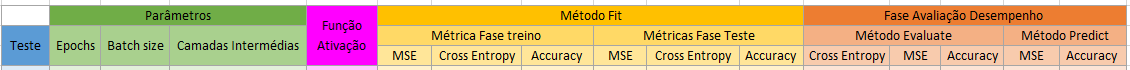
\includegraphics[scale=0.7]{Imagens/tabela.png}
    \caption{Informações registadas em cada cenários de teste e topologia de Rede exploradas}
    \label{fig:Tabela}
\end{figure}

O sumário dos resultados estará descrito através de uma tabela, caracterizada pelo formato visível na figura \ref{fig:Tabela} e que apresenta a seguinte estrutura:
\begin{itemize}[noitemsep]
    \item Cada coluna representa um parâmetro relevante no processo de treino ou teste da rede, como o número de \textit{Epochs}, \textit{Batch Size}, topologia da rede ou métricas de avaliação conseguidas; 

    \item Na coluna \textit{Camadas Intermédias}:
    \begin{itemize}[noitemsep]
        \item O número de camadas intermédias definidas é dado pelo comprimento do vetor;
        
        \item O número de nodos de cada camada, é dado pelo valor do índice \textit{i} que representa essa camada;
        
        \item Camadas de Dropout são identificadas pela letra \textit{D}. 
    \end{itemize}
    
    \item As \textit{Métricas da Fase Teste} dentro da opção \textit{Método Fit} (a amarelo) representam as avaliações nos cenários em que no método fit se utilizou o parâmetro \textit{Percentage split} com valor 0.33;
    
    \item A secção laranja, representa a avaliação do desempenho da rede, através dos métodos predict e evaluate disponibilizados na plataforma keras. 
    
    Em ambos as funções referidas é utilizado o mesmo dataset de teste, previamente criado e não utilizado em fase de treino. 
\end{itemize}

\newpage
\begin{figure}[H]
    \centering
    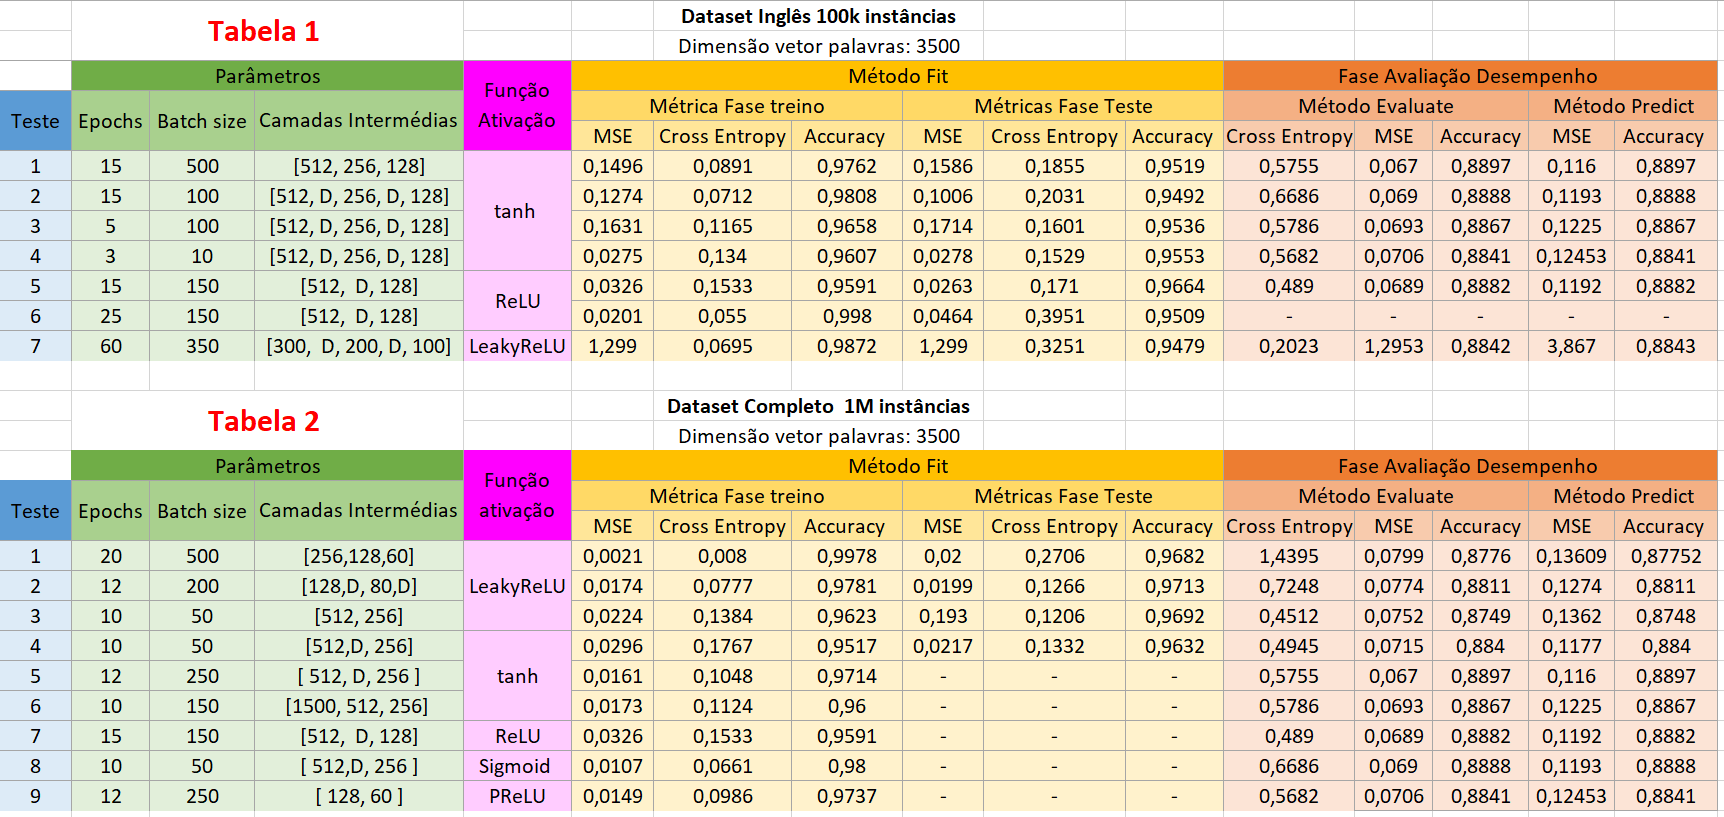
\includegraphics[scale=0.62, angle=90]{Imagens/tabelas.png}
    \caption{Tabelas com os parâmetros e resultados dos cenários de avaliação de desempenho das RNAs criadas.}
    \label{fig:tabelas}
\end{figure}

\section{Dataset completo \textit{Tweets}}

A Tabela 1 da Figura \ref{fig:tabelas} descreve os resultados os cenários de treino de RNAs realizados sobre a versão reduzida do dataset. 

Focando alguns dos resultados obtidos:
\begin{itemize}
    \item Numa primeira abordagem ao dataset completo, foram desde logo utilizadas algumas considerações destacadas nas secções \ref{sec:ParametrostreinoRede}.
    
    Para o Teste 1, foi inicialmente criada uma topologia de rede com 3 camadas intermédias, tendo cada uma delas, respetivamente, 256 e 128 e 60 neurónios. 
    
    Na tentativa de obter rapidamente bons resultados, utilizou-se como forma de inicialização dos pesos o método de \textit{Xavier} e como funções de ativação dos neurónios de cada camada selecionou-se a função LeakyReLU. 
    
    Foram realizadas 20 passagens pelos dados, alimentando a rede com 500 instâncias a cada iteração do treino. 
    
    \begin{figure}[H]
        \hspace{-0.4in}
        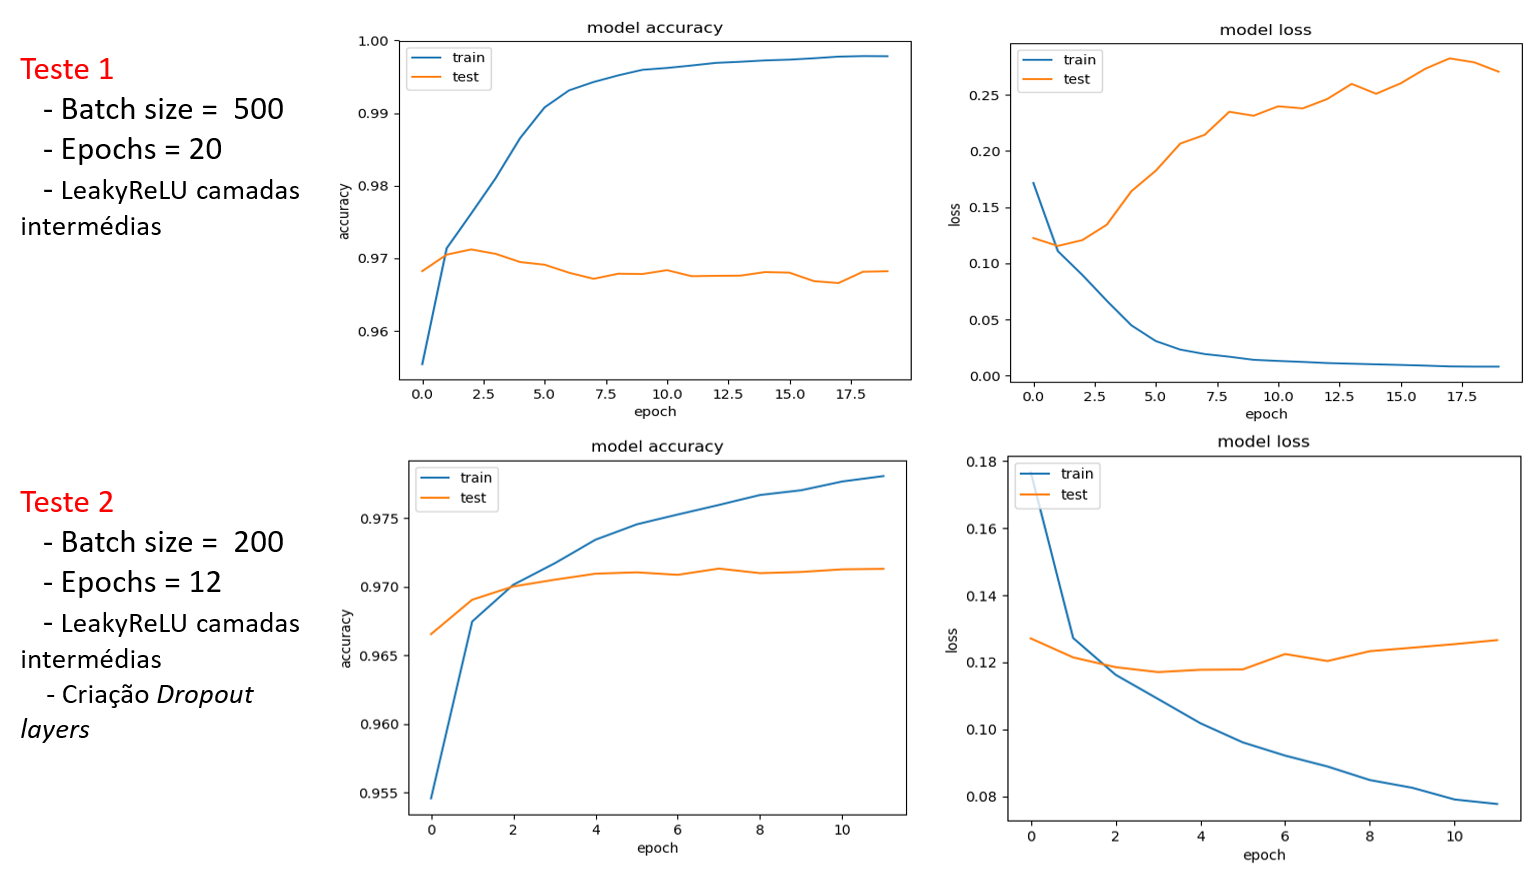
\includegraphics[scale=0.65]{Imagens/t37.png}
        \caption{Resultados Teste 1 e 2, com uso do dataset completo para criação de conjuntos de treino + teste.}
        \label{fig:teste1}
    \end{figure}
    
    Estes resultados (Figura \ref{fig:teste1}) tornam-se relevantes no sentido em que, apresentam desde logo um cenário de overfitting. A accuracy da rede no final da fase de treino apresenta-se na casa dos 99\% e, na fase de teste, atinge apenas os 88\%. 
    
    Na tentativa de reduzir este sobre ajustamento aos dados, no Teste 2 procurou-se introduzir camadas de \textit{Dropout} na rede e simplificar a sua complexidade, reduzindo a topologia para duas camadas com, respetivamente, 128 e 80 nodos. 
    
    Apesar destas alterações reduzirem o valor de \textit{accuracy} em fase de treino, o valor de 97\% continua relativamente superior face aos 88\% novamente obtidos na fase de teste. 
    
    \item Independente da função de ativação utilizada nas camadas intermédias da rede, mesmo que o seu contradomínio não se apresente entre [-1, 1], como no caso da ReLU ou da Sigmoide, foi mesmo assim possível obter uma taxa de acertos de cerca de 88\% em fase de Teste da RNA. 
    (Relembrando que o output deve ser -1, 0 ou 1, conforme a classificação de um texto num sentimento negativo, neutro ou positivo) 
    
    Estes resultados permitem observar que as camadas intermédias são capazes de generalizar a informação que analisam, mesmo que não propaguem entre si sinais com valores negativos. 
    
    Ao longo das iterações de treino, as sinapses das camadas intermédias com estas funções ReLU ou Sigmoide não transmitem valores negativos, porque o seu contradomínio é positivo. Contudo, o peso das ligações (\textit{W}) pode eventualmente ajustar-se para valores negativos, sendo assim capazes de influenciar a aprendizagem da rede a ajustar-se inevitavelmente aos dados. 
    
    \item Relativamente ao Teste 7, foi utilizada uma topologia de rede com 3 camadas intermédias, possuindo 300, 200 e 100 neurónios, respetivamente. 
    Foi também a inicialização dos pesos com o método de \textit{Xavier} e utilizada a função LeakyReLU.  
    
    \begin{figure}[H]
        \hspace{-0.4in}
        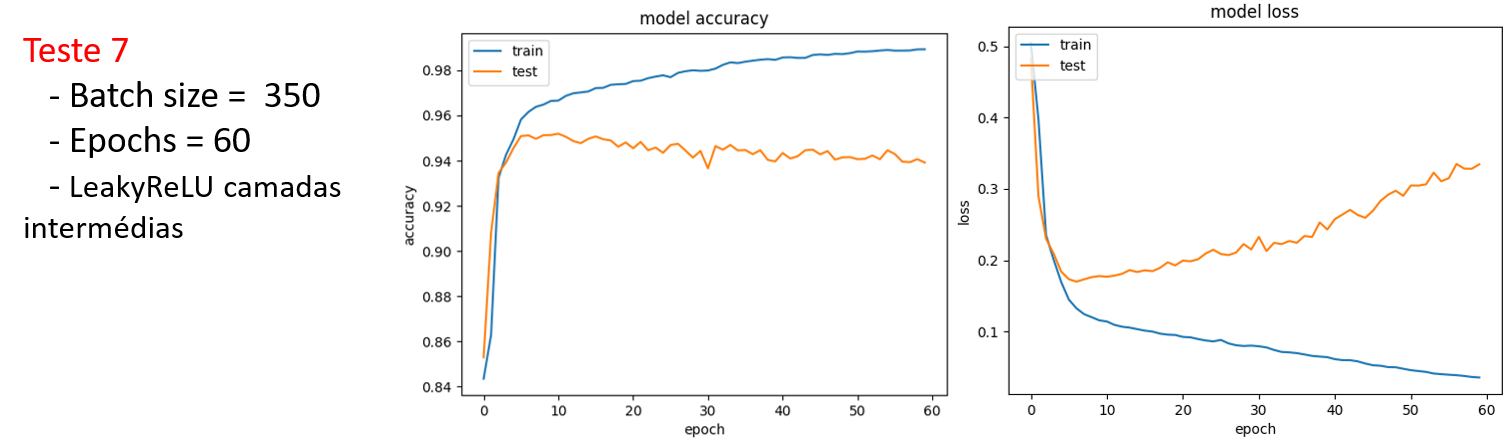
\includegraphics[scale=0.65]{Imagens/t7.png}
        \caption{Resultados do Teste 7, com uso do dataset completo para criação de conjuntos de treino + teste.}
        \label{fig:teste4}
    \end{figure}
    
    A análise dos resultados conseguidos com esta arquitetura e apresentados na Figura \ref{fig:teste4} é interessante devido à evolução das curvas a cada \textit{Epochs}. 
    
    O surgimento de picos (altos e baixos em \textit{accuracy}) ao longo das diferentes \textit{Epochs} permite concluir que com estas configurações, a função de ativação ou as métricas de avaliação não são as mais indicadas. 
    Isto porque, num determinado \textit{Epoch}, a atualização dos gradientes através da métrica \textit{Loss} definida leva a bons resultados mas, num \textit{Epochs} seguinte, os resultados já não são favoráveis. 
    
    \item No geral, independente da topologia ou parâmetros utilizados, os valores de accuracy em fase de teste, com dados exclusivamente reservados para treino, rondam sempre os 88\%. 
\end{itemize}
    

\section{Dataset \textit{Tweets} em Inglês}

A Tabela 2 da Figura \ref{fig:tabelas} descreve os resultados os cenários de treino de RNAs realizados sobre a versão reduzida do dataset e segue a mesma estrutura descrita na secção anterior.

Relembrando, este conjunto de dados contem apenas publicações em inglês e, por apresentar menores dimensões, permite explorar vetores de palavras com maiores dimensões e redes com maior complexidade, pois dá mais folga a nível dos recursos de memória necessários para o analisar.

Apenas descrevendo alguns dos principais resultados obtidos: 

\begin{itemize}
    \item Numa primeira abordagem (Teste 1 e 2), foi utilizada uma topologia de rede com 3 camadas intermédias, tendo cada uma delas, respetivamente, 512, 256 e 128 neurónios. 

    Como funções de ativação utilizou-se a função tangente hiperbólica \textit{tanh} e os pesos das ligações foram inicializados com uma distribuição uniforme. 
    
    \begin{figure}[H]
        \hspace{-0.4in}
        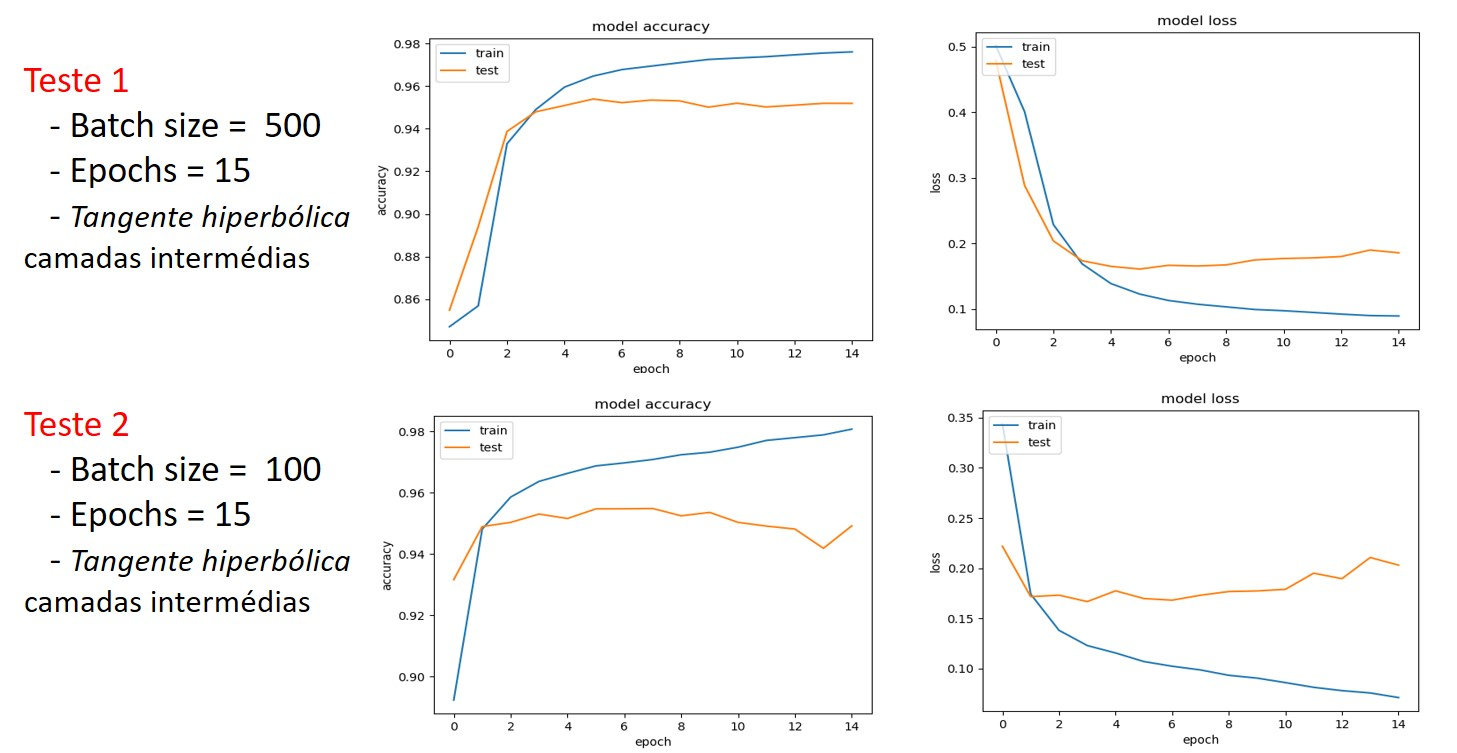
\includegraphics[scale=0.67]{Imagens/teste1.jpg}
        \caption{Resultados Teste 1 e Teste 2 com o dataset reduzido apenas com publicações em inglês}
        \label{fig:teste2}
    \end{figure}
    
    Observando os gráficos da Figura \ref{fig:teste2}, as retas descreverem inicialmente um cenário de overfitting, onde os valores de \textit{accuracy e cross entrophy (loss)} na fase de treino se apresentam ligeiramente superiores face à fase de avaliação de desempenho. 

    No Teste 2, realizar um teste com o mesmo número de \textit{epochs} (15) mas reduzindo o parâmetro \textit{batch size} de 500 para 100 exemplos contribuiu apenas para acentuar ligeiramente os resultados de \textit{overfitting} já assinalados. 
    
    O crescimento suave da curva de \textit{accuracy} na fase de treino, permite assumir que a função de ativação e avaliação internas da rede levam a um correto ajustamento dos pesos a cada iteração, permitindo assim uma aprendizagem gradual, sem grandes variações entre cada \textit{Epoch}.
    
    \item Reduzir o número de \textit{Epochs} para um valor abaixo das dezenas (Teste 3 e Teste 4) não permite nenhuma avaliação concreta ao desempenho de aprendizagem da rede. 
    As informações dos gráficos nestes cenários não são suficientes para compreender a evolução da rede na fase de treino. 
    
    Contudo, as métricas devolvidas foram registadas e enquadram-se dentro dos resultados dos restantes testes. 
    
   \item Relativamente ao Teste 6, foi aumentado o número de \textit{Epochs}, procurando tirar o melhor partido possível da função de ativação \textit{ReLU}. 
   
   Contudo, o maior número de \textit{Epochs} permitiu apenas aumentar o efeito de \textit{overfitting} já visualizado noutros cenários de treino. A accuracy a nivel de treino manteve-se próxima dos 88\%.
   
   \begin{figure}[H]
        \hspace{-0.4in}
        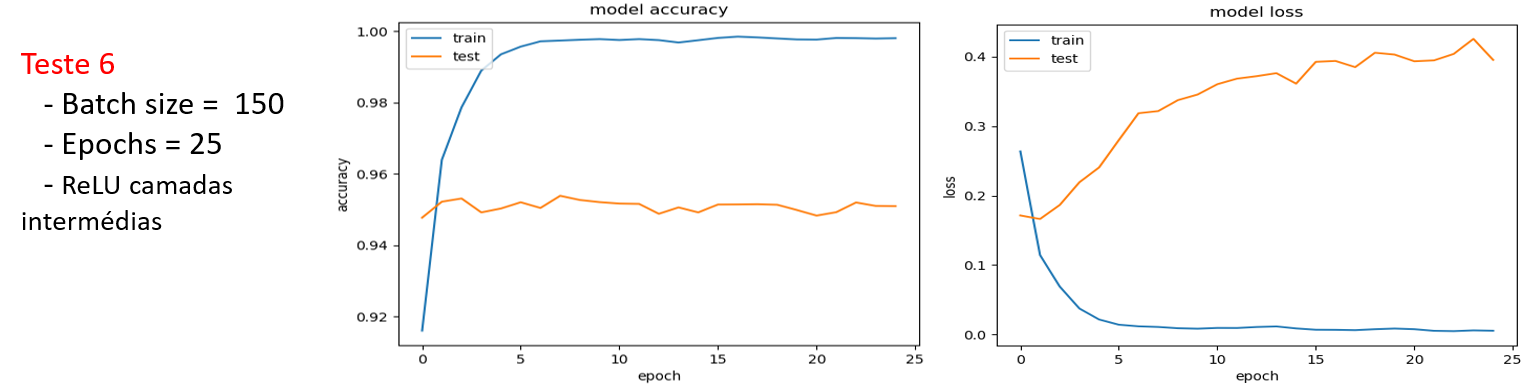
\includegraphics[scale=0.65]{Imagens/t2.png}
        \caption{Resultados Teste 6, com o  dataset reduzido apenas com publicações em inglês}
        \label{fig:teste3}
    \end{figure}
   
\end{itemize}
\chapter{Conclusão e Trabalho Futuro}
\label{chp:conclusao}

Depois de analisados e descritos os princípios e algumas metodologias Ágeis, constata-se que estas trouxeram melhorias notórias nos processos e fluxos de trabalho das empresas, que se convertem em maior organização, capacidade de produção e consequentemente, satisfação dos clientes. É de notar também que, apesar do que muitas pessoas possam imaginar, estas metodologias não são propriamente recentes. Já foram inventadas há alguns anos, mas só começaram a popularizar-se na área da produção de Software há relativamente pouco tempo e o seu uso tem vindo a tornar-se cada vez mais comum. Apesar das vantagens das abordagens mais Ágeis, elas têm vantagens e desvantagens e não servem para todo o tipo de projeto.\\
Na nossa opinião o método desenvolvido tem algumas características que à partida definimos como prioritárias: é simples, não demora muito a responder, é direto e ajuda a ter uma primeira perceção do método de trabalho a seguir.\\
É também importante definir que esta é apenas uma primeira versão do método de diagnóstico, será esperado que como trabalho futuro se sugira uma segunda parte do questionário que apenas seja respondida se a primeira parte indicar que o projeto deva seguir uma abordagem ágil, e onde se consiga perceber em específico que método Ágil o projeto deve seguir. Para além disso, e devido ao facto de o desenvolvimento deste projeto ter sido feito num contexto académico com prazos limitados, é também importante validar as questões num contexto real em projetos já desenvolvidos e onde se consiga ter uma perceção se as abordagens ágeis ou tradicionais resultaram.


\appendix


\bibliographystyle{plain}
\bibliography{Bibliografia}

\end{document}